% CERRA empirical systems paper: editable working draft, 29 September 2026.
% Main document: main.tex. Compile with pdfLaTeX (Overleaf default).
\documentclass[10pt,twocolumn,letterpaper]{article}
\usepackage[T1]{fontenc}
\usepackage[utf8]{inputenc}
\usepackage[margin=0.78in,columnsep=0.27in]{geometry}
\usepackage{lmodern,microtype,amsmath,amssymb,graphicx,booktabs,tabularx,array,longtable}
\usepackage{enumitem,xcolor,eso-pic,fancyhdr}
\usepackage{tikz}
\usetikzlibrary{arrows.meta,positioning}
\usepackage{hyperref}
\definecolor{ink}{HTML}{183C50}
\definecolor{teal}{HTML}{087E8B}
\hypersetup{colorlinks=true,linkcolor=ink,citecolor=ink,urlcolor=teal,
 pdftitle={Beyond Answer Accuracy: Evaluating Source-Grounded Language-Model Assistants in Interactive Transportation Analytics},
 pdfauthor={Authors to be confirmed},pdfsubject={CERRA empirical systems research draft}}
\setlength{\emergencystretch}{2em}
\setlength{\tabcolsep}{4pt}
\setlist{nosep,leftmargin=*}
\raggedbottom
\pagestyle{fancy}\fancyhf{}
\fancyhead[L]{\small CERRA: Interactive assistant evaluation}
\fancyhead[R]{\small Working draft}
\fancyfoot[C]{\thepage}
\setlength{\headheight}{14pt}
\renewcommand{\headrulewidth}{0.3pt}
\newcommand{\config}[1]{\textsf{#1}}
\newcommand{\pp}{percentage points}
\title{\vspace{0.3in}\textbf{Beyond Answer Accuracy: Evaluating Source-Grounded Language-Model Assistants in Interactive Transportation Analytics}}
\author{Author names, order, and affiliations to be confirmed}
\date{Research manuscript draft --- 29 September 2026}
\begin{document}
% Required ARA landscape badge: first page only, 2.2 cm wide, clear of title.
\AddToShipoutPictureFG*{%
  \AtPageUpperLeft{%
    \put(0,0){%
      \makebox[0pt][l]{%
        \hspace*{\dimexpr\paperwidth-0.78in-2.2cm\relax}%
        \raisebox{-0.27in}[0pt][0pt]{%
          \raisebox{-\height}[0pt][0pt]{%
            \href{https://www.agenticresearch.sh/ara/cnpcshangbo/ara-cerra-assistant-benchmark}{%
              
\includegraphics[width=2.2cm]{figures/ara-badge.png}}}}}}}

}
\twocolumn[{\maketitle
\begin{abstract}
Language-model assistants embedded in analytical dashboards must do more than return plausible answers: they must query the intended data, preserve unrequested interface state, and respect the limits of the evidence. We study these requirements in CERRA, a transportation analytics application with Maryland crash-data and Baltimore high-injury-network workflows. A frozen suite contains 24 primary tasks and four controls, each repeated three times per configuration. Five evaluation campaigns cover ten model configurations and eleven configuration--campaign observations, yielding 924 application attempts. Evaluation combines independent source-derived oracles, structured-plan checks, observed browser effects, and identity-blind, AI-assisted narrative review. In a contemporaneous local comparison, Qwen3.8 27B achieves 63/72 strict successes versus 49/72 for Qwen3 14B: a paired difference of 19.4 percentage points, with a 95\% task-cluster bootstrap interval of [1.4, 38.9]. Median request latency rises from 3.77 to 14.50 seconds, while observed UI-state violations fall from 3/21 to 0/21 primary browser attempts. A separate GPT-6.1 Sol API extension records 64/72 strict successes and a 2.15-second median; its distinct execution conditions and absence of a contemporaneous comparator preclude an isolated model ranking. Failure analysis separates state violations from schema failures, missing qualifications, ambiguous task wording, and failures whose model-versus-application origin cannot be isolated. The results motivate reporting workflow correctness, state preservation, and latency together, while preserving the boundary between configuration observations and causal claims about model generations.
\end{abstract}
\par\vspace{0.8em}
\noindent\textbf{Keywords:} language-model evaluation; analytical assistants; tool use; human--AI interaction; transportation analytics; reproducibility.
\vspace{1.3em}}]

\section{Introduction}
Natural-language interfaces can make analytical dashboards easier to approach, but they also change what correctness requires. A user who asks for the number of crash reports matching current filters may expect records outside the visible map to count. A request to clear the year should preserve every other selection. A question about next month's fatal-crash probability cannot be answered from historical counts alone. In each case, fluent language is compatible with an incorrect system outcome.

These issues are especially visible in transportation analysis, where similar terms can refer to different geographical units, missing observations should not be interpreted as negative evidence, and descriptive counts do not establish exposure-normalized risk or causal effects. An assistant may also change the analytical state from which a user draws subsequent conclusions. Assessing the response text alone can therefore miss both useful behavior and consequential failures.

We investigate this problem in CERRA, an existing web application that connects language-model assistants to Maryland crash data and Baltimore high-injury-network (HIN) source products. Its assistants use language models to select constrained operations and, for some tasks, narrate evidence. Shared application code validates plans, queries data, renders answers, and applies supported filter changes. The relevant unit of evaluation is the entire configured assistant, including these surrounding components.

Our research questions are:
\begin{enumerate}
\item \textbf{RQ1:} How do configured assistants perform when success requires correct source use, task intent, narrative qualifications, and actual interface effects together?
\item \textbf{RQ2:} In a contemporaneous local comparison, how does higher strict task success relate to response time and repeated-task consistency?
\item \textbf{RQ3:} Which distinctions are lost when strict failures are summarized by a single accuracy number?
\end{enumerate}

We contribute a documented evaluation design for a bounded analytical workflow; an empirical account of ten configurations across five campaigns; and a failure audit that distinguishes contract violations from practical state changes and evidential errors. The contemporaneous Qwen comparison is the main paired study. Historical deployments and a separate API extension provide application context, with their distinct execution conditions retained. We do not pool them into a controlled leaderboard.

The study is deliberately limited. Its tasks were authored with implementation knowledge, narrative judgments are AI-assisted rather than expert-validated, and the model configurations differ in more than model family. These limitations are part of the evaluation design and interpretation, not reasons to hide failed attempts or replace the frozen primary score.

\section{Related Work}
\paragraph{Multi-dimensional model evaluation.}
HELM argues for evaluating language models across standardized scenarios and multiple metrics rather than accuracy alone~\cite{helm}. Our study applies this broad principle to a narrower application: correctness must be considered alongside interaction effects and latency. We do not reproduce HELM's coverage or assess its other dimensions, such as fairness and calibration.

\paragraph{Agents in executable environments.}
AgentBench evaluates language models through interactions with executable environments~\cite{agentbench}. WebArena emphasizes realistic web environments and functional task outcomes~\cite{webarena}. These approaches motivate measuring the state that an interaction actually produces. CERRA differs from an unrestricted web agent: its model selects application-defined operations, while shared code performs validation, data access, and UI execution. The resulting evaluation concerns bounded application assistance rather than autonomous navigation across arbitrary websites.

\paragraph{Tool use and repeated reliability.}
$\tau$-bench evaluates tool--agent--user interaction using domain constraints and resulting database states, including reliability across repeated trials~\cite{taubench}. We likewise retain state and repeat-task outcomes, but use a fixed suite, three repetitions, and the directly observed number of tasks passing all three. We do not equate that count with a separately estimated general reliability metric.

\paragraph{Application-relevant comparisons.}
Kapoor et al. identify evaluation practices that can obscure practical agent performance and advocate comparisons relevant to downstream use~\cite{agentsmatter}. Our response is to identify configurations and execution environments explicitly, preserve all attempts, and separate historical deployments from a contemporaneous pair. We measure time, but not monetary cost or energy. The contribution is a transparent domain case study, not a claim that these evaluation principles originate here.

\section{System and Evaluation Boundary}
\subsection{Two analytical workflows}
The Maryland module supports queries over crash-report records, their temporal and geographic filters, ambient weather, contributor fields, and original or estimated map locations. The study uses frozen read-only indexes derived from the application's source snapshots. Public Maryland State Police dashboards describe data that may be revised or differ across reporting systems~\cite{mdsp}; consequently, our oracles refer to the retained application snapshot, not a later live total.

The Baltimore HIN module exposes source-derived corridor, intersection, tract, and severe-injury records, together with documentary context. Tasks include rankings at specified corridor-length thresholds, source-ranked intersection selection, missing-value handling, and qualifications about scoring units or documentary disagreements. The six hashed exports cover ranked corridors at 0.5-, 1-, and 2-mile minimum lengths; the database Top300Intersections product; severe-injury and non-motorist segments; tract attributes with 2020 Census TIGER/Line geometry; and a source-version audit. Retained methodology notes identify the documentary source as ``UMD/BCDOT Draft Final Report, September 2025.'' This is a retained source label, not a separately verified full report title. These are tests of faithful access to the retained products. They do not validate the underlying HIN methodology, crash-location estimates, or any countermeasure's effectiveness.

\subsection{A constrained model--application pipeline}
Figure~\ref{fig:system} defines the system boundary. A request contains a question, current UI context, and where needed a canonical conversation history. The assistant routes the request through existing prechecks, a model planner, validation and any normal internal repair, deterministic data operations, and answer rendering. Some HIN responses include generated narration. Supported actions are applied by the browser; the evaluator inspects the resulting state.

Correct numeric output can arise because the model routed a question to the correct deterministic computation. It is not evidence that the model performed the arithmetic. Conversely, a bad final plan or answer can arise from shared reconciliation or rendering logic. Unless raw intermediate evidence isolates the cause, we report an application failure without assigning it exclusively to the foundation model.

\begin{figure*}[t]
\centering
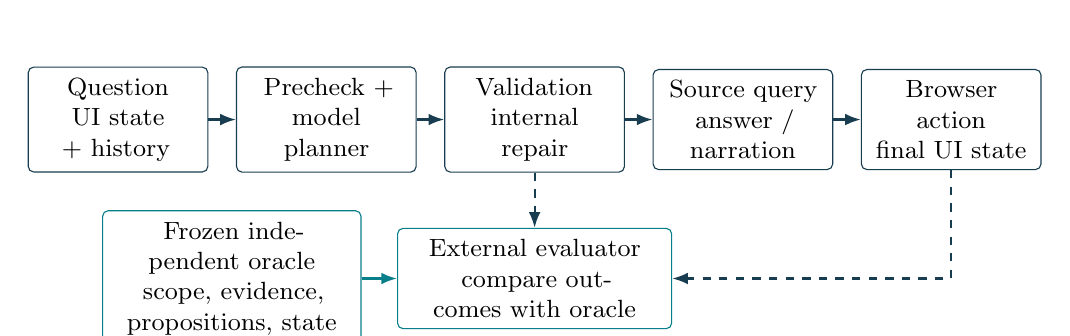
\begin{tikzpicture}[font=\small,node distance=0.35cm,
 box/.style={draw=ink,rounded corners=2pt,align=center,minimum height=0.85cm,text width=2.0cm,inner sep=4pt},
 arr/.style={-{Latex[length=2mm]},thick,draw=ink}]
\node[box] (request) {Question\\UI state + history};
\node[box,right=of request] (plan) {Precheck +\\model planner};
\node[box,right=of plan] (validate) {Validation\\internal repair};
\node[box,right=of validate] (data) {Source query\\answer / narration};
\node[box,right=of data] (ui) {Browser action\\final UI state};
\draw[arr] (request)--(plan);\draw[arr] (plan)--(validate);\draw[arr] (validate)--(data);\draw[arr] (data)--(ui);
\node[box,draw=teal,below=0.7cm of validate,text width=3.2cm] (eval) {External evaluator\\compare outcomes with oracle};
\node[box,draw=teal,left=0.45cm of eval,text width=3.0cm] (oracle) {Frozen independent oracle\\scope, evidence, propositions, state};
\draw[arr,teal] (oracle.east)--(eval.west);
\draw[arr,dashed] (validate.south)--(eval.north);
\draw[arr,dashed] (ui.south)|-(eval.east);
\end{tikzpicture}
\caption{Evaluation boundary. The configured assistant includes the model, shared application logic, data operations, and browser effects. The oracle is available to the evaluator, not provided to the evaluated model. Some refusal controls terminate in shared prechecks.}
\label{fig:system}
\end{figure*}

\section{Tasks, Oracles, and Metrics}
\subsection{Frozen task suite}
The suite contains 24 primary tasks and four controls. Each configuration is evaluated three times per task. Primary categories are Maryland data queries (nine tasks), HIN source queries (five), HIN reasoning and limitations (three), supported UI filter changes (five), and ambiguous or unsupported UI actions (two). Three primary prompts are in Chinese; no language-specific comparative claim is made from this small subset. The compact inventory in Appendix~\ref{app:tasks} identifies each task.

Nine of the 28 tasks are browser cases: seven primary tasks and two controls. The other 19 use the same authenticated API payloads as the UI. Thus each configuration--campaign observation contains 72 primary attempts and 12 controls, including 27 browser attempts. Five campaigns retain all 924 scheduled application attempts: 792 primary and 132 control, or 297 browser and 627 API attempts. These attempts are not 924 independent questions or necessarily 924 individual model generations. Shared prechecks may answer without inference, and internal validation repair or separate narration may invoke inference more than once.

The controls are reported separately. MD16 tests a shared deterministic refusal; MD18, HIN01, and HIN11 are previously shown reference examples. None enters the primary score, primary latency, or paired model-ranking inference. A control answered by deterministic shared logic supplies no evidence of a model-quality difference.

\subsection{Independent oracles and state preservation}
Before inference, task records freeze the prompt, initial state, history, expected operation and scope, source-derived numeric or record-level expectations, required narrative propositions, and allowable browser effects. Follow-up tasks use a canonical prior context instead of the result of another benchmark attempt. The evaluated model receives the normal application request fields, not task IDs, gold plans, or scoring notes.

Maryland tasks include independently recorded read-only SQL anchors. For HIN, numeric oracles were computed in a separate Python pass over the frozen application JSON exports, without importing the application query, answer-rendering, reconciliation, or model code. This establishes computational independence from the evaluated path, not independent data collection or validation of the upstream extraction process. The oracle is independent of the response being judged. A returned plan that agrees with its own evidence is insufficient if both use the wrong county, temporal range, viewport scope, or source unit. Browser tasks also require the intended action to occur and unrelated state to remain unchanged. For an ambiguous or unsupported action, a successful refusal or clarification must preserve the current state.

\subsection{Strict success and diagnostic outcomes}
For model configuration $m$, primary task $i$, and repetition $r$, let $y_{mir}\in\{0,1\}$ denote strict success. A pass requires the expected HTTP completion, correct selected-model identity, permitted operation and scope, required constraints and evidence, required narrative propositions, and expected browser effects. Missing an essential requirement fails the attempt. Optional qualifications are not promoted to requirements after observing an answer.

The strict rubric distinguishes contractual correctness from observed state changes. An extra action field can fail even if it redundantly repeats the current value. We therefore separately count \emph{UI-state violations}: observed value changes that violate the frozen task policy among the 21 primary browser attempts per configuration. The five supported filter tasks also have their own 15-attempt success denominator. A 422 response is an application validation failure, not a transport outage. The paired MD17 violation applies a requested year change prematurely, before resolving the ambiguous geography; it does not imply that the year value was itself unrequested.

With $T=24$ tasks and $R=3$ repetitions, the primary score is
\begin{equation}
 S_m=\frac{1}{T}\sum_{i=1}^{T}\bar y_{mi},\qquad
 \bar y_{mi}=\frac{1}{R}\sum_{r=1}^{R}y_{mir}.
\end{equation}
Every task has equal weight. Because all tasks have three repetitions, the score also equals primary passes divided by 72. We report the number of tasks passing all three repetitions as an additional directly observed consistency measure.

A secondary functional-equivalence analysis credits narrowly specified cases that satisfy a practical interpretation despite a strict mismatch. This analysis was post-hoc in the original campaign and inherited by subsequent campaigns. It never replaces strict success; reporting both exposes sensitivity to the interface contract.

\subsection{Uncertainty and timing}
For a contemporaneous pair $a,b$, the paired effect is
\begin{equation}
 \widehat\Delta_{b-a}=\frac{1}{T}\sum_{i=1}^{T}(\bar y_{bi}-\bar y_{ai}).
\end{equation}
We use 10,000 paired task-cluster bootstrap resamples, retaining all repetitions within each sampled task, and percentile 95\% intervals. Marginal score intervals likewise resample each configuration's 24 task means. The single-configuration API extension has a marginal interval but no paired effect estimate. The scheduling/bootstrap seed is 20260918. It does not fix token sampling. These unadjusted intervals describe suite-dependent uncertainty; repeated attempts are not treated as independent task draws, and the convenience sample does not justify population-wide significance claims.

Request latency measures the complete application request, including model loading, internal retries, and data access. Median and 90th-percentile (P90) values include all primary attempts, including failures. Browser completion adds the final UI render and is reported separately. We also count strict successes completed within 30 seconds; for browser tasks, this criterion uses browser completion time. Controls remain excluded.

\subsection{Narrative review and audit history}
Generated HIN narratives receive identity-blind, AI-assisted proposition review. The reviewer receives the frozen required and forbidden propositions and the answer, while model identities and aggregate results are withheld. Structural and semantic requirements must both pass. Across the five campaigns, 132 narrative-review records are retained. This is single-reviewer AI assistance, not human expert validation or an inter-rater reliability study. The original campaigns' retained review receipts do not identify the reviewer model/provider, model snapshot, or tool version; this missing metadata limits exact adjudication replay. The API extension records a separate Codex reviewer context, but its exact backend model snapshot/version is not exposed. Context separation supplies procedural separation, not independent human expertise or independence of model training.

The September 29 local-pair review used the original notes, supplied evidence, and four anonymous historical judgments for calibration, without consulting identities, aggregate results, or external resources. The API-extension reviewer received only the anonymized instruction, response, and calibration files, preserving the same scoring notes and historical interpretation. The reviewer did not inspect trial keys, model identities, current-run summaries, or network resources.

Audit history matters for reproducibility. The original campaign added an aggregation layer after freezing to enforce model-identity and browser-evidence requirements already present in the written protocol; original and protocol grades were preserved. Separately, the September 24 narrative packet initially omitted original scoring notes. Re-review of unchanged answers with complete notes and anonymous calibration changed 15 of 24 judgments. The revised packet was carried into the September 29 study. We report final audited scores while retaining initial artifacts. These facts support a frozen written rubric, but not a claim that every analysis implementation or review packet was preregistered without amendment.

\section{Experimental Campaigns}
\subsection{Historical production observations}
The September 18 campaign evaluates Qwen3 8B, Llama 3.1 8B, and Gemma 3 4B in production v36. Their engines and loading policies differ. Qwen3 uses a resident BF16 Transformers configuration with temperature 0.7, top-$p$ 0.8, and top-$k$ 20. Llama and Gemma use Ollama Q4\_K\_M packages with temperature 0.1 and cold-loading behavior. These are practical configurations, not a controlled model-size comparison.

The September 23 campaign evaluates GPT-4.1 mini, GPT-5.4 mini, and GPT-5.4 through the OpenAI Responses API in production v48. Planner calls request JSON-object output with an additional JSON-only instruction, per-call output-token budgets, a 60-second model-call timeout, and storage disabled. Temperature, reasoning effort, and inference seed are not explicitly supplied. Provider aliases are not immutable weight snapshots.

The September 24 campaign evaluates Qwen3 14B and Gemma 4 12B. Additive provenance identifies the actual v51/v52 deployments as sharing the same application archive and environment revision; it supersedes the initial v50 manifest label. An independent source audit preceded inference, although one machine-readable source receipt was captured shortly after the first attempt. The paper preserves these details instead of presenting a cleaner but inaccurate chronology.

All campaigns retain the same task objects, analysis plan, and acceptance constraints. Calls are sequential and reset to frozen context. Three-model campaigns rotate first, middle, and last position within tasks. Two-model campaigns alternate model order, balancing positions over the schedule but not perfectly within each three-repetition task. No external retry replaces a failed attempt. Prompts, generation settings, oracles, and written strict criteria remain unchanged during inference; the audit-layer changes are described above.

\subsection{Contemporaneous local Qwen comparison}
The September 29 study compares \config{qwen3:14b} with \config{qwen3.8:27b-q4\_K\_M}. It reuses the historical application base, frozen data, and all 28 task records, with local routing and timeout additions. Five Maryland database hashes and six HIN JSON hashes match the retained historical source snapshot. The nine Maryland numeric/source oracles were independently replayed. The two package digests are retained in the paper's provenance inventory.

Both configurations use Ollama 0.34.3, Q4\_K\_M quantization, temperature 0.1, an 8192-token context setting, disabled thinking, and \texttt{keep\_alive=0}. They share an RTX 5090 with 32 GB memory; the resident production Qwen3 8B and camera processes remain active. Partial CPU offload for Qwen3.8 is observed in a connectivity smoke check. Speculative decoding is not explicitly configured; runtime option resolution implies it is disabled, but it is not separately measured per trial.

Each repetition uses a seeded task shuffle. Within a task, model order alternates according to the fixed case index and repetition index. Each model is first in 42 of the 84 task--repetition pairs. The run retains all 168 outcomes, 54 browser records, and 24 narrative reviews. It executes a local compiled Worker rather than traversing the public production-site network path.

Architecture, parameter count, memory residency, and offload differ between the two configurations. Consequently, the comparison estimates a practical configuration difference under shared conditions. It cannot isolate a release-generation effect, and its latency should not be interpreted as a controlled baseline for earlier production measurements.

\subsection{September 29 API extension}
\label{sec:api-extension}
A fifth campaign evaluates \config{gpt-6.1-sol}, displayed as GPT-6.1 Sol, through the OpenAI Responses API. It uses an isolated compiled copy of the same historical application base and the retained source snapshots. The preflight audit matches five Maryland database hashes, six HIN export hashes, and the nine original Maryland oracle payloads; structural-grader parity is checked against 588 historical attempts. Only the model catalog and OpenAI transport receive the new routing and configuration. Planner and narration prompts, validators, internal repair, task objects, source oracles, and written strict scoring remain unchanged.

The configuration explicitly requests medium reasoning effort, an 8,192-token total output budget, a 60-second model-call timeout, and disabled storage. The output budget includes both reasoning and visible output; it is not an 8,192-token answer-length target. Existing concise-answer prompts remain in force. Temperature is not supplied, and planner calls retain JSON-object output. The provider route is the regional US Responses endpoint. Provider receipts account for 93 calls during scored application attempts, all reporting the requested \config{gpt-6.1-sol} alias; separate smoke calls are excluded. This alias is not an immutable weight snapshot.

This is a single-configuration extension: 24 primary tasks and four controls are each evaluated three times, with the inherited seeded task shuffles. All 84 application outcomes, 27 browser records, and 12 narrative reviews are retained and verified. It has no contemporaneous comparator and produces no within-campaign paired model-difference estimate. Request latency includes the frozen application's work and remote API calls, while browser completion also includes the resulting interface update. These timings have a different execution path from both earlier public production requests and local Ollama inference. Explicit reasoning effort and the combined output budget also differ from the historical API configurations. Cross-campaign score and timing differences are therefore descriptive observations of practical configurations, not equal-compute comparisons or isolated model-generation effects.

\section{Results}
\subsection{Workflow success across campaigns (RQ1)}
Table~\ref{tab:all-results} reports eleven configuration--campaign observations across five campaigns. Strict success ranges from 34/72 to 66/72 across the historical production configurations, but the broad intervals and environment differences preclude an intrinsic ranking. For example, Qwen3 8B passes 51/72 overall yet succeeds on only 6/15 supported filter attempts, illustrating why aggregate correctness cannot substitute for an interaction-specific result.

Gemma 4 12B records 58/72 strict successes, 15/15 supported filter successes, and no observed UI-state violations in its 21 primary browser attempts. Its paired advantage over Qwen3 14B in the September 24 campaign is 9.7 points, with interval [$-8.3$, 29.2]. GPT-5.4 records 66/72 primary successes, but its 11.1-point advantage over GPT-5.4 mini has interval [$-4.2$, 26.4]. Neither interval excludes zero; descriptive ordering should not be presented as a conclusive superiority claim.

Across all five campaigns, recorded HTTP outcomes comprise 883 status-200 responses and 41 status-422 responses. Successful HTTP delivery does not imply strict task success. A completed request can select the wrong scope, omit a required qualification, or change state incorrectly.

% Generated by make_figures.py from 5 verified campaign summaries.
% Requires graphicx and booktabs; intended for a two-column manuscript.
\begin{table*}[t]
\centering
\caption{11 observations from 10 CERRA assistant configurations across 5 campaigns. Strict and functional scores use 72 primary attempts per observation; controls are excluded. Intervals are 95\% task-cluster bootstrap intervals. Request latency retains failed primary attempts. Runtime paths and dates differ between campaigns.}
\label{tab:all-results}
\small
\setlength{\tabcolsep}{5pt}
\resizebox{\textwidth}{!}{%
\begin{tabular}{@{}lrrrrrrr@{}}
\toprule
Configuration & Strict success & 95\% CI & Median (s) & P90 (s) & UI actions & UI-state violations & Functional \\
\midrule
\multicolumn{8}{@{}l}{\textit{September 18, 2026 --- Production site}} \\
Qwen3 8B & 51/72 (70.8\%) & 52.8--87.5 & 1.06 & 2.17 & 6/15 & 6/21 & 51/72 \\
Llama 3.1 8B & 40/72 (55.6\%) & 36.1--75.0 & 2.00 & 3.77 & 14/15 & 7/21 & 40/72 \\
Gemma 3 4B & 34/72 (47.2\%) & 27.8--66.7 & 2.40 & 4.18 & 12/15 & 3/21 & 48/72 \\
\addlinespace[4pt]
\multicolumn{8}{@{}l}{\textit{September 23, 2026 --- Production site}} \\
GPT-4.1 mini & 57/72 (79.2\%) & 62.5--93.1 & 1.20 & 2.59 & 12/15 & 3/21 & 63/72 \\
GPT-5.4 mini & 58/72 (80.6\%) & 65.3--93.1 & 1.12 & 2.76 & 14/15 & 0/21 & 62/72 \\
GPT-5.4 & 66/72 (91.7\%) & 79.2--100.0 & 1.27 & 2.94 & 12/15 & 0/21 & 66/72 \\
\addlinespace[4pt]
\multicolumn{8}{@{}l}{\textit{September 24, 2026 --- Production site}} \\
Qwen3 14B & 51/72 (70.8\%) & 54.2--87.5 & 2.93 & 5.56 & 12/15 & 3/21 & 57/72 \\
Gemma 4 12B & 58/72 (80.6\%) & 63.9--95.8 & 3.51 & 6.71 & 15/15 & 0/21 & 61/72 \\
\addlinespace[4pt]
\multicolumn{8}{@{}l}{\textit{September 29, 2026 --- Paired local}} \\
Qwen3 14B & 49/72 (68.1\%) & 50.0--84.7 & 3.77 & 7.20 & 11/15 & 3/21 & 55/72 \\
Qwen3.8 27B Q4\_K\_M & 63/72 (87.5\%) & 75.0--100.0 & 14.50 & 29.81 & 15/15 & 0/21 & 63/72 \\
\addlinespace[4pt]
\multicolumn{8}{@{}l}{\textit{September 29 API extension --- Frozen local app / API}} \\
GPT-6.1 Sol & 64/72 (88.9\%) & 76.4--100.0 & 2.15 & 4.88 & 15/15 & 0/21 & 64/72 \\
\bottomrule
\end{tabular}}
\par\vspace{3pt}
\begin{minipage}{\textwidth}\footnotesize
UI actions: supported filter changes. UI-state violations: actual value changes violating the frozen task policy among 21 primary browser attempts; redundant unchanged fields are excluded. Functional equivalence was a post-hoc diagnostic in the initial campaign, inherited by later campaigns; it does not replace strict success. The September 29 paired-local baseline is the contemporaneous Qwen3 14B rerun. Campaigns that share a date remain separate experiments; the API extension is not part of this Qwen pair.
\end{minipage}
\end{table*}


\subsection{A separate API configuration observation}
GPT-6.1 Sol passes 64/72 primary attempts (88.9\%), with a 95\% task-cluster interval of [76.4\%, 100\%]. Twenty-one of the 24 tasks pass all three repetitions. All 15 supported filter attempts and all 21 primary browser attempts pass, with zero observed UI-state violations. The twelve controls and twelve identity-blind narrative assessments also pass; controls remain outside the primary score. The inherited functional-equivalence sensitivity remains 64/72, so it adds no passes to this configuration's strict score.

Median request latency is 2.15 seconds and P90 is 4.88 seconds; median primary-browser completion is 7.04 seconds. All 64 strict successes finish within the 30-second budget. These measurements describe the frozen local-application/API route in Section~\ref{sec:api-extension}, not a matched speed comparison with other campaigns. All 84 requests return HTTP 200, but eight primary attempts fail strict scoring: three on MD01, three on MD04, and two on MD09. This contrast isolates the difference between successful request delivery and successful analytical assistance. Neither the score nor the latency establishes superiority over the historical GPT configurations or local models without a contemporaneous comparison.

\subsection{Paired quality--latency trade-off (RQ2)}
Figure~\ref{fig:paired} presents the contemporaneous pair. Qwen3.8 27B passes 63/72 primary attempts (87.5\%) versus 49/72 (68.1\%) for Qwen3 14B. The paired difference is 19.4 points, with interval [1.4, 38.9]. The observed fixed-suite difference favors the newer, larger configuration, and the interval remains above zero under empirical task-cluster resampling. This describes sensitivity to the tested task mix, not a sampled deployment population or an isolated model-generation effect.

The number of tasks passing every repetition increases from 15/24 to 21/24. Supported filter success rises from 11/15 to 15/15. UI-state violations fall from 3/21 to 0/21 primary browser attempts; all three baseline violations are premature partial actions on the ambiguous Baltimore task discussed below. Zero observed UI-state violations on seven tasks is not evidence of universal safe automation.

This improvement comes with longer response times. Median request latency increases from 3.77 to 14.50 seconds, and P90 from 7.20 to 29.81 seconds. Median browser completion increases from 8.70 to 15.50 seconds. With a 30-second completion budget, strict successes are 49/72 for the baseline and 55/72 for Qwen3.8, compared with 49/72 and 63/72 without that budget. Thus eight of the newer configuration's strict successes finish after the deadline. This is a descriptive view of service usefulness, not an independently validated user-tolerance threshold.

Both models produce 69/72 status-200 primary responses and three 422 failures, so HTTP completion alone conceals their success difference. Controls score 9/12 and 12/12, respectively, and are excluded from the paired inference.

\begin{figure*}[t]
\centering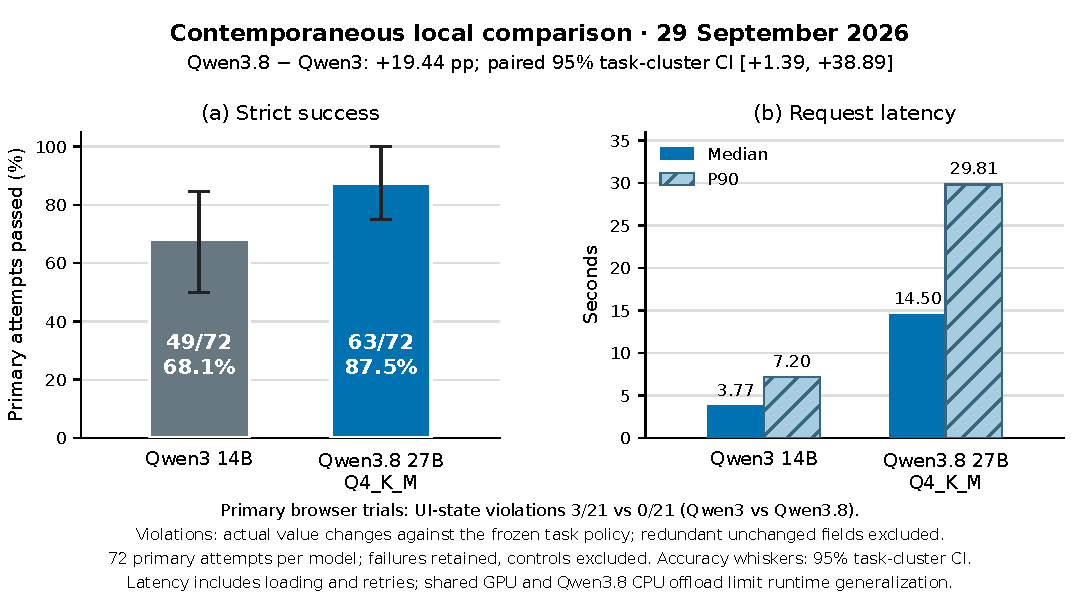
\includegraphics[width=0.96\textwidth]{figures/paired-results.pdf}
\caption{September 29 contemporaneous local comparison. Left: strict primary success with 95\% task-cluster bootstrap intervals. Right: median and P90 request latency over all 72 primary attempts per configuration. The paired success difference is 19.4 points [1.4, 38.9]. Historical production latency is not included in this figure.}
\label{fig:paired}
\end{figure*}

\subsection{Differences by task family}
For the paired comparison, both configurations pass all 15 HIN source-query attempts. HIN reasoning and limitation checks improve from 8/9 to 9/9. Maryland data queries improve from 15/27 to 18/27, while boundary tasks improve from 0/6 to 6/6. Supported filter actions improve from 11/15 to 15/15. The improvement is therefore distributed unevenly and does not eliminate data-query failures.

These category counts are diagnostic subdivisions of the same small suite. They are not independent experiments, and we do not assign category-level significance claims. Repeated failure on a single task contributes three failures, emphasizing the importance of reviewing the task-level records.

\section{Failure Analysis (RQ3)}
\subsection{Actual state violations versus strict patch failures}
MD17 asks to focus the map on ``Baltimore'' for 2020, without specifying City or County. The baseline changes the year from 2024 to 2020 in all three attempts before resolving the geographical ambiguity. Qwen3.8 preserves state and requests clarification. The year change is explicitly requested, but applying it before geographical clarification violates the frozen preserve-state policy. These are premature partial actions under that policy; the experiment does not establish user harm or show that the year itself was unrequested.

By contrast, one baseline RV01 attempt includes redundant action fields whose values match existing controls. It fails the strict requirement to change only the requested fields, but produces no unwanted value change. Collapsing both phenomena into an ``unsafe action'' total would overstate the latter's observed effect. Strict contract adherence and actual mutation should remain separately inspectable.

On MD15, both configurations refuse an unsupported rain/fatal map filter and preserve state. The baseline nevertheless fails all three strict attempts because it omits the required explanation that weather can be queried but cannot be applied as that map filter. This is a missing capability qualification, not an unintended action.

\subsection{Correct displayed values can still fail the contract}
For MD05, both configurations display the correct count of 14,220 rain-associated crash reports in the requested 2022 statewide snapshot. The baseline chooses a disallowed breakdown operation instead of an accepted summary/weather operation, causing three strict failures. Describing this as numerical fabrication would be false. The inherited functional-equivalence sensitivity credits such narrowly defined cases without modifying the primary rubric.

Under that secondary analysis, the baseline improves from 49/72 to 55/72 and Qwen3.8 remains 63/72. The primary 19.4-point difference becomes an 11.1-point descriptive difference under the secondary interpretation. The primary paired interval should not be reused for this different estimand. The earlier Gemma 3 campaign shows an even larger sensitivity, moving from 34/72 to 48/72. These examples show that a structured interface contract is a consequential evaluation choice.

\subsection{Task ambiguity and shared application constraints}
MD04 asks for Baltimore County report totals for all years and all severity levels. Both paired configurations return the correct aggregate, 151,679, with appropriate filters. The frozen oracle expects separate annual rows, whereas the prompt does not explicitly require one row per year. Both fail all three strict attempts. The API extension repeats this pattern: the aggregate is correct in all three attempts, but the required annual rows are absent. We retain the scores and flag the ambiguity rather than retrospectively rewriting the oracle.

MD01 tests counting the complete current selection, including records outside the viewport. Every configuration--campaign observation fails all three attempts on this task. In the paired study, the baseline's final plan uses a selected-record path with zero evidence, while Qwen3.8 returns an unsupported outcome without the required evidence. In the API extension, all three final plans use viewport scope and display zero rather than the frozen selection's 266 reports.

The frozen application's scope-reconciliation code contains a confirmed shared defect: for plans reaching its scope-assignment branch, a keyword check matches ``visible'' without handling negation or exclusion. It therefore assigns viewport scope even for ``outside the visible map,'' overwriting an otherwise appropriate filtered scope. This constraint is already recorded in the frozen task metadata and remains unchanged during evaluation. MD01 is consequently not a model-only failure. The shared rule is known, while the raw pre-reconciliation plans are not retained; we cannot reconstruct each model's original interpretation or isolate its additional contribution to every failed path.

MD09 accounts for the API extension's other two failures. The application can compare original and estimated placements under the frozen task, but two responses select an unsupported operation. The third repetition passes the required evidence and caveat checks. This is a repeated-task inconsistency on a supported capability, not a transport error. All eight extension failures remain in the primary score and timing distribution.

MD07 is a regression: the baseline passes the selected-crash weather interpretation, while Qwen3.8 produces three 422 responses. MD12 shows the reverse pattern for clearing only the year restriction. Missing raw planner traces prevent a narrower diagnosis such as malformed JSON or a particular internal repair failure. The observable result is application validation failure on a supported task.

\subsection{Narrative limitations remain part of correctness}
The paired narrative review accepts 20 of 24 reviewed responses. Three failures are baseline control HIN11 responses missing the people-versus-crashes unit distinction in the HIN formula; one primary HIN12 response makes an unsupported claim about documentary or ranking consistency. The separate API extension passes all twelve narrative reviews under the inherited rubric. These outcomes illustrate why source grounding includes units and uncertainty, not only matching numbers. They remain dependent on the stated AI-assisted review procedure and require human verification before strong domain conclusions are drawn. Passing a small known set of limitation questions does not establish general scientific reasoning ability.

\section{Discussion}
\subsection{Deployment selection is a policy choice}
A default model balances latency, observed task behavior, and the consequences of failure. The largest strict score does not automatically determine the best default for an interactive demonstration. The current deployment selects Gemma 4 12B as a practical local default and makes the tested Qwen3.8 configuration optional. The former's historical 58/72 score, 3.51-second median, complete supported-filter performance, and zero observed UI-state violations informed that choice. Qwen3.8 offers higher strict success in its own paired study with substantially longer latency.

This is an operational decision under incomplete evidence. There is no contemporaneous Qwen3.8--Gemma 4 paired experiment, no measured utility function, and no user study establishing a preferred waiting time. The current default should be revisited using matched conditions, broader tasks, and direct user feedback. We do not label it a statistically established optimum.

\subsection{Design implications for analytical assistants}
First, preserve state unless the requested action is both supported and unambiguous. A partial action can silently alter subsequent analysis even when the accompanying text acknowledges a limitation. Second, expose and test the boundary between a queryable attribute and an actionable filter; these capabilities need not coincide. Third, make source units and missingness explicit, particularly when users ask for risk, causality, or future outcomes beyond the evidence.

For evaluation, retain both contract-level and practical diagnostics. A strict score supplies a reproducible acceptance boundary, while mutation counts, HTTP outcomes, displayed-value checks, and reviewed narrative propositions explain what the score means. This recommendation follows from observed distinctions; the present study does not test whether a proposed UI redesign or new validator resolves them.

\section{Threats to Validity}
\paragraph{Task selection and coverage.}
The suite is small, authored with application knowledge, and not sampled independently from user traffic. Controls contain previously shown examples. Exact task reuse enables comparison but also creates a narrow fixed target. The study does not establish robustness to paraphrase distributions, multilingual use generally, adversarial inputs, or unseen analytical domains. Wide intervals reflect limited task coverage but do not correct selection bias.

\paragraph{Configurations and execution conditions.}
Weights, precision, parameter count, adapters, prompts, sampling, loading policy, and hosting conditions vary. Historical campaigns use different application deployments and a public network path. The contemporaneous pair reduces some variation, but its models differ in size and offload on a shared GPU. The API extension uses a frozen local application, a regional remote endpoint, explicit medium reasoning effort, and a different combined reasoning/output budget. These conditions do not supply a matched comparison with either historical API deployments or the Qwen pair. Backend alias drift limits exact replay of hosted models. Timing includes loading and application work and is not a token-generation throughput measure.

\paragraph{Measurement and adjudication.}
The frozen rubric contains at least one wording/granularity ambiguity and distinguishes extra fields more strictly than visible harm. Narrative assessment lacks independent human raters. A corrected packet materially changed earlier judgments, and some enforcement code was added after the written protocol freeze. These changes are documented, but the work should not be described as an externally preregistered trial. Structural graders do not exhaustively validate every surplus prose assertion or source label.

\paragraph{Attribution and statistical scope.}
Shared preprocessing and postprocessing can dominate outcomes. Final artifacts do not always include raw model intermediates. The study therefore attributes effects to configurations and avoids isolated causal claims. Bootstrap intervals are unadjusted and dependent on this convenience suite; the number of repetitions is too small to characterize rare failures or long-run consistency precisely. No inference cost, energy consumption, human productivity benefit, or crash-risk reduction was measured.

\section{Reproducibility and Research Practice}
The retained research archive contains frozen manifests, exact contexts and histories, source-derived oracles, code and data hashes, package identifiers, request outcomes, browser evidence, review decisions, and additive audit notes. Appendix~\ref{app:provenance} identifies the campaign manifests. Aggregated figures in this draft are reproducible from the included CSV and plotting script; they introduce no new inference runs.

The public \href{https://github.com/cnpcshangbo/ara-cerra-assistant-benchmark/tree/v0.1.0}{CERRA benchmark artifact (v0.1.0)} provides all 28 original question strings, fixed contexts, scoring rules, frozen grader code, relevant application snapshots, and sanitized per-attempt outcomes supporting offline aggregate reconstruction. A \href{https://github.com/cnpcshangbo/ara-cerra-assistant-benchmark/blob/v0.1.0/review/README.md}{questions-first review packet} includes answer keys, known ambiguities, and a blank feedback worksheet; human expert review remains pending. One selected-record task (MD07) uses a documented public placeholder. Exact end-to-end reruns require the retained source data, record binding, application environment, and browser harness; raw answers, individual source records, credentials, and private operational traces are not redistributed. The website remains access-controlled. The first-page badge links to the \href{https://www.agenticresearch.sh/ara/cnpcshangbo/ara-cerra-assistant-benchmark}{project-specific ARA}, which records bounded claims and their evidence. Code and review materials are MIT-licensed; the manuscript retains author rights.

This draft was assembled with AI assistance from experiment artifacts. Authorship, affiliations, funding, acknowledgments, disclosure wording, and the target venue require author confirmation. Independent domain review and a fresh held-out task suite are appropriate next research steps; neither is represented as completed here.

\section{Conclusion}
Evaluating a language-model assistant inside an analytical dashboard requires checking the complete workflow: intended data scope, independent evidence, required qualifications, and actual state changes. In CERRA's fixed suite, a contemporaneous Qwen3.8 27B configuration improves strict success over Qwen3 14B while substantially increasing latency. A separate GPT-6.1 Sol API campaign records 64/72 strict successes despite every request returning HTTP 200. Its unmatched execution conditions limit cross-campaign inference. The failure audit shows why neither HTTP completion nor a single strict score fully describes practical behavior. Transparent separation of configuration effects, rubric sensitivity, and pipeline uncertainty makes these bounded results useful for deployment decisions without turning them into an unsupported general model ranking.

\begin{thebibliography}{9}
\bibitem{helm} P. Liang et al. Holistic Evaluation of Language Models. \emph{Transactions on Machine Learning Research}, 2023. \url{https://openreview.net/forum?id=iO4LZibEqW}.
\bibitem{agentbench} X. Liu et al. AgentBench: Evaluating LLMs as Agents. In \emph{International Conference on Learning Representations}, 2024. \url{https://arxiv.org/abs/2308.03688}.
\bibitem{webarena} S. Zhou et al. WebArena: A Realistic Web Environment for Building Autonomous Agents. In \emph{International Conference on Learning Representations}, 2024. \url{https://arxiv.org/abs/2307.13854}.
\bibitem{taubench} S. Yao, N. Shinn, P. Razavi, and K. Narasimhan. $\tau$-bench: A Benchmark for Tool-Agent-User Interaction in Real-World Domains. In \emph{International Conference on Learning Representations}, 2025. \url{https://arxiv.org/abs/2406.12045}.
\bibitem{agentsmatter} S. Kapoor, B. Stroebl, Z. S. Siegel, N. Nadgir, and A. Narayanan. AI Agents That Matter. \emph{Transactions on Machine Learning Research}, 2025. \url{https://openreview.net/forum?id=Zy4uFzMviZ}.
\bibitem{mdsp} Maryland Department of State Police. Interactive Data Dashboards. Accessed September 29, 2026. \url{https://mdsp.maryland.gov/safety-prevention/interactive-data-dashboards}.
\end{thebibliography}

\clearpage\onecolumn\appendix
\section{Task Inventory}\label{app:tasks}
Descriptions below are compact paraphrases, not replacements for the frozen prompts and initial contexts. A dagger marks one of the three Chinese prompts, translated here for readability. ``Browser'' denotes an observed UI task; other tasks use the application API. Controls remain outside all primary score and latency denominators.
\small
\begin{longtable}{@{}p{0.075\textwidth}p{0.11\textwidth}p{0.085\textwidth}p{0.67\textwidth}@{}}
\toprule ID & Family & Mode & Task and principal acceptance boundary\\\midrule\endfirsthead
\toprule ID & Family & Mode & Task and principal acceptance boundary\\\midrule\endhead
MD01 & Data query & API & Count the full current crash selection, including reports outside the visible map.\\
MD02 & Data query & API & Summarize statewide ambient-weather completeness across all years.\\
MD03 & Data query & API & Produce statewide county-by-county totals for 2021, without severity restriction.\\
MD04 & Data query & API & Tabulate Baltimore County totals for all years and severities; frozen oracle requires annual rows (wording ambiguity noted).\\
MD05 & Data query & API & Count 2022 statewide crash reports listing ambient rain.\\
MD06 & Data query & API & Resolve a follow-up ``What about 2025?'' using the frozen canonical history.\\
MD07 & Data query & API & Explain whether an unmarked weather-contributor field on a selected crash establishes clear weather.\\
MD08 & Data query & API & Describe GPS screening for visible crashes without overstating positional certainty.\\
MD09 & Data query & API & Compare original and estimated locations in the viewport and count reports entering or leaving.\\
MD10$^{\dagger}$ & UI action & Browser & Filter 2021 Baltimore County serious-injury crashes.\\
MD11 & UI action & Browser & Filter 2022 Anne Arundel fatal or serious-injury crashes.\\
MD12 & UI action & Browser & Remove only the year restriction; preserve other selections.\\
MD15 & UI boundary & Browser & Handle unsupported rain/fatal filtering; explain the query/filter distinction and preserve state.\\
MD17 & UI boundary & Browser & Clarify ambiguous ``Baltimore'' before acting on a 2020 map request.\\
RV01 & UI action & Browser & Change only county and severity; preserve year, GPS, estimates, and map positions.\\
RV02 & UI action & Browser & Clear only GPS cross-check while preserving estimate filters and comparison positions.\\
HIN02 & HIN source & API & Return the three half-mile-minimum corridors with the largest source fatality counts.\\
HIN03 & HIN source & API & Return the first three Tier 2 intersections in source-rank order.\\
HIN05 & HIN source & API & Rank four tracts by households without vehicles, excluding unavailable values.\\
HIN06$^{\dagger}$ & HIN source & API & Count all Major Concern severe-injury source records, ignoring current map filters.\\
HIN10$^{\dagger}$ & HIN source & API & Resolve a follow-up switching to the two-mile-minimum corridor group, retaining top-three scope.\\
HIN12 & HIN limits & API & Qualify conflicting intersection influence distances and differences between public and application rankings.\\
HIN13 & HIN limits & API & Decline an unsupported forecast of next-month fatal-crash probability per vehicle-mile.\\
HIN14 & HIN limits & API & Decline an unsupported causal percentage reduction from a hypothetical North Avenue road diet.\\
\midrule
MD16 & Control & Browser & Deterministic refusal: rain cannot be established as causing fatal crashes per mile from these data.\\
MD18 & Control & Browser & Previously shown example: 2023 Baltimore City fatal-crash filtering.\\
HIN01 & Control & API & Previously shown example: retrieve the five highest-ranked one-mile corridors.\\
HIN11 & Control & API & Previously shown example: explain HIN scoring, including people-versus-crashes units.\\
\bottomrule
\end{longtable}

\normalsize

\clearpage
\section{Provenance and Audit Inventory}\label{app:provenance}
The aggregate package is derived from the final audited summaries of the following retained campaigns. Campaign and model hashes are listed in \texttt{provenance.json}; source-export hashes are listed in \texttt{data-provenance.json}; abbreviated hashes below are human-readable identifiers, not substitutes for full integrity checking. Dates are local Maryland campaign labels, not unique experiment identifiers. The local Qwen pair and the API extension have distinct campaign folders and manifest hashes despite sharing a date.
\begin{center}\small
\begin{tabularx}{\textwidth}{@{}lXlll@{}}
\toprule Campaign & Archive directory & Trials & Manifest SHA-256 prefix & Context\\\midrule
Sep.\ 18 & \texttt{transportation-model-benchmark-2026-09-18} & 252 & \texttt{a73f5b9e835ec776} & Production v36\\
Sep.\ 23 & \texttt{transportation-gpt-benchmark-2026-09-23} & 252 & \texttt{9239d992da1869f9} & Production v48\\
Sep.\ 24 & \texttt{local-model-benchmark-2026-09-24} & 168 & \texttt{a2fb59169c45f215} & Production v51/v52\\
Sep.\ 29 & \texttt{qwen-newer-benchmark-2026-09-29} & 168 & \texttt{a32cb875e9e9b2ac} & Compiled local app\\
Sep.\ 29 & \texttt{gpt61-sol-benchmark-2026-09-29} & 84 & \texttt{b2777e4a29be6c55} & Frozen local app / API\\\bottomrule
\end{tabularx}\end{center}
Both September 29 campaigns use application base \texttt{6ed65fc06f525e8bbe8cb800ce80487642f6120a}, with separately retained routing/configuration changes. The paired local run spans 14:17:05--14:50:59 UTC; the API extension spans 23:50:47--23:58:05 UTC on September 29, 2026. Qwen3 14B package digest begins \texttt{bdbd181c33f2ed1b}; Qwen3.8 27B Q4\_K\_M begins \texttt{25b843619e944cd0}. The API extension records the provider-reported alias and frozen runtime settings rather than a weight digest. Final verification accounts for all scheduled attempts, browser records, and narrative decisions. Package digests identify tested local artifacts; family names alone do not.

\paragraph{Audit distinctions to preserve when revising.}
Keep the contemporaneous 49/72 Qwen3 14B baseline separate from its historical 51/72 observation. Do not merge control results with primary results, apply the primary uncertainty interval to secondary scores, call 422 responses network outages, or infer raw planner behavior from final postprocessed records. Narrative review is AI-assisted, and the September 24 correction is part of the record. Data correctness concerns the retained snapshot, not external epidemiological validity.

\paragraph{Author review before submission.}
Confirm author order and affiliations; verify all narrative judgments with independent domain reviewers; choose a venue and adapt its template and disclosure rules; decide what sanitized evaluation artifacts can be released; and add a held-out evaluation if claiming generalization beyond this implementation-aware suite. These items describe unfinished research or administrative work, not completed results.
\end{document}
